\myChapter{Motivation}\label{chap:introduction}
Moderne Unternehmens- und Webanwendungen zu entwickeln ist ein komplexes Thema
und die dabei verwendeten Technologien unterliegen einem ständigen Wandel. Das
folgende Kapitel soll diese Anwendungen genauer charakterisieren und
den Rahmen sowie den Aufbau dieser Arbeit vorstellen.

\section{Unternehmensanwendungen}
Hierfür ist es zuerst notwendig die Art von Anwendungen festzulegen, die im
Folgenden näher behandelt werden sollen. Der Begriff Unternehmensanwendung
(\emph{Enterprise Applications}) umfasst grundsätzlich eine Art von Software,
für die es zwar keine allgemein gültige Definition gibt, die aber einige
charakteristische Merkmale aufweist (siehe \cite{fowler:2002} S. 3).

Grundsätzlich werden in einer Unternehmensanwendung \emph{große Mengen an Daten}
verarbeitet und auch \emph{dauerhaft gespeichert}. Für die dauerhafte Speicherung
kommen normalerweise eine oder mehrere Datenbanken zum Einsatz und die Menge der
Daten erreicht dabei oft einige Terabyte oder mehr. Normalerweise wird auf diese
Daten dann auch von \emph{vielen verschiedenen Benutzern}, häufig gleichzeitig,
zugegriffen. Je nach Anzahl der Benutzer kann diese Eigenschaft auch besondere
Anforderungen an die Skalierbarkeit eines Systems stellen. Durch die Menge der
von der Anwendung verarbeiteten Daten ist es auch wahrscheinlich, dass die
\emph{Benutzeroberfläche sehr umfangreich} ist und in viele unterschiedliche
Ebenen oder Fenster aufgeteilt ist. Weiterhin erfordert die Umsetzung der
Anforderungen und Geschäftsprozesse oft eine \emph{komplexe Anwendungslogik}.
Das ist vor allem der Fall, wenn Sonderfälle berücksichtigt werden müssen, die nicht
direkt einem verallgemeinerten Geschäftsprozess folgen. Ein weiteres Merkmal ist,
dass eine Unternehmensanwendung in den meisten Fällen mit anderen Anwendungen
kommuniziert. Im Umkehrschluss heißt das auch, dass die Anwendung selbst
wahrscheinlich eine Reihe von Schnittstellen bereitstellen muss, die die
Kommunikation mit anderen Anwendungen erlauben.

Beispiele für Unternehmensanwendungen sind Warenwirtschaftssysteme,
Buchhaltunssysteme, Content Management Systeme oder eine
Patientenaktenverwaltung\footnote{Keine Unternehmensanwendungen sind: Embedded
Systems, Text- oder Bildverarbeitungsprogramme, Betriebssysteme, Compiler oder
Videospiele}. Da viele dieser Systeme eine Weboberfläche anbieten fallen auch ein
Großteil der Webapplikationen unter diese Kategorie. Im weiteren Verlauf sollen
die Begriffe \emph{Anwendung} und Unternehmensanwendung gleichbedeutend
verwendet werden.

Um der Komplexität bei der Entwicklung von Unternehmensanwendungen
entgegen zu wirken wird zur Strukturierung häufig eine
\emph{Schichtenarchitektur} verwendet. Eine Schichtenarchitektur erlaubt es,
eine Anwendung in logische Schichten zu unterteilen, wobei immer eine übergeordnete Schicht die
Schnittstelle der direkt darunterliegenenden Schicht benutzt. Die
darunterliegende Schicht stellt diese Schnittstelle zur Verfügung, hat aber
selbst keine Kenntnis von den übergeordneten Schichten. Dadurch können die
einzelnen Schichten einer Anwendung relativ getrennt voneinander behandelt
werden, was die Komplexität deutlich reduziert. In \cite{fowler:2002} (vgl. S.
20) wird eine Unternehmensanwendung in die drei grundlegenden Schichten
\emph{Datasource}, \emph{Application Logic} und \emph{Presentation} unterteilt.
Diese Unterteilung soll auch hier für den Aufbau einer Anwendung verwendet
werden. Tabelle \ref{tab:basiclayers} zeigt eine Übersicht der Schichten und
deren Aufgaben.

\begin{table}[h] \begin{tabularx}{\textwidth}{lX} \toprule
	\tableheadline{Schicht} & \tableheadline{Beschreibung} \\
	\midrule
	Presentation / Remoting & Stellt die Anwendungslogik für einen Benutzer
	bereit. Beispielsweise über eine grafische Benutzeroberfläche oder als Services
	für entfernte Methodenaufrufe \\
	\midrule
	Application Logic & Beinhaltet die eigentliche Anwendungslogik \\ 
	\midrule
	Datasource &
	Stellt die Verbindung zu Datenbanken oder anderen
	entfernten Systemen her	\\
	\bottomrule
	\end{tabularx}
	\caption{Übersicht über die drei grundlegenden Schichten}
	\label{tab:basiclayers}
\end{table}

Abbildung \ref{ill:eaoverview} zeigt die Einordnung einer Unternehmensanwendung
mit den vorgestellten Schichten in einem beispielhaften Gesamtzusammenhang. Darin
wird die Kommunikation in eine Client und eine Serverseite unterteilt. Auf der
Serverseite steht die Anwendung selbst und die entfernten Systeme mit welchen sie
kommuniziert, beispielsweise eine Datenbank oder eine andere
Unternehmensanwendung. Auf der Clientseite stehen die Anwendungen, die wiederum
mit der Anwendung selbst kommunizieren. In diesem Beispiel handelt es sich um
eine andere Unternehmensanwendung und einen Webserver, der die Daten der
Anwendung für die Darstellung in einem Webbrowser aufbereitet. Diese Aufgabe
könnte aber auch von der Anwendung selbst direkt in der Presentation Schicht
übernommen werden.

\begin{figure}
    \center{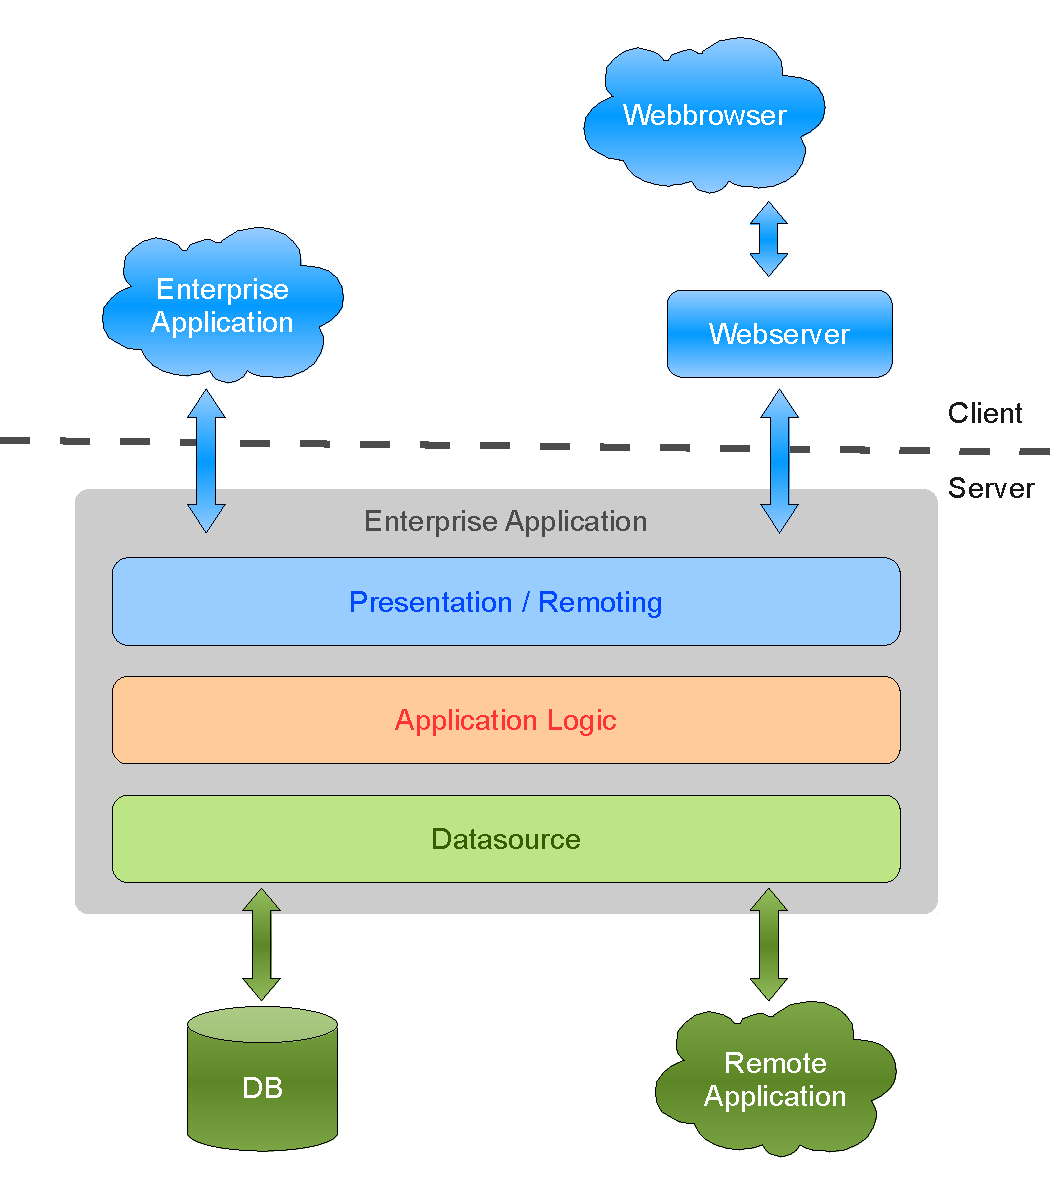
\includegraphics[width=\linewidth]{images/overviews/ea_overview}}
	\caption{Einordnung einer Unternehmensanwendung}
	\label{ill:eaoverview}
\end{figure}

\section{Aufgaben}
Die in dieser Arbeit vorgestellten Implementierungen sind grundsätzlich in zwei
Aufgabenbereiche unterteilt.

Im ersten Teil soll auf Grundlage der oben aufgezeigten Merkmale von
Unternehmensanwendungen der Service Layer vorgestellt werden. Es handelt sich
hierbei um einen Teil der Application Logic Schicht der dazu dient einer
übergeordneten Schicht eine eindeutige und einheitliche Schnittstelle zur
Anwendungslogik bereitzustellen. Damit haben die verschiedenen
Darstellungsmöglichkeiten der Presentation Schicht dann eine einzige gemeinsame
Schnittstelle zur Verfügung. Ferner sollen Funktionalitäten dieses Service Layer
herausgearbeitet und implementiert werden, die entsprechend den allgemeinen
Merkmalen einer Unternehmensanwendung in verschiedenen Anwendungen für die
Grundlage eines Service Layer verwendet werden können.

Der zweite Teil befasst sich mit der Presentation Schicht, genauer dem Teil,
der die Aufgabe übernimmt die Funktionalitäten des Service Layer über entfernte
Methodenaufrufe zur Verfügung zu stellen. Deshalb soll dieser Teil der
Presentation Schicht im weiteren Verlauf auch \emph{Remoting} Schicht genannt
werden. Aufgabe ist es hier ein abstraktes Modell für die Darstellung von Service
Methoden und Methodenaufrufen zu erstellen und einen zentralisierten
Ausführungsmechanismus für diese zu entwickeln. Darauf aufbauend sollen nun
eine Reihe von Protokollen für entfernte Methodenaufrufe evaluiert werden und
die jeweiligen Implementierungen, die den vorher entwickelten zentralen
Ausführungsmechanismus verwenden, realisiert werden.

\section{Herangehensweise}
Auch wenn der Schwerpunkt dieser Arbeit in der Anwendungslogik (Application
Logic) und Remoting Schicht liegt ist es für das Verständnis des Gesamtsystems
sinnvoll die Schichtenarchitektur einer Anwendung in ihrer Gesamtheit zu
betrachten. Für die hier verwendete Architektur wurden dazu die drei
grundlegenden Schichten weiter unterteilt, wobei die einzelnen Komponenten im
weiteren Verlauf der Arbeit vorgestellt werden sollen.

Nach der Behandlung wichtiger Grundlagen in Kapitel \ref{chap:basics} wird in
Kapitel \ref{chap:datasourcelayer} die Schicht des Datasource- und Domain Layer
näher vorgestellt. Der Datasource Layer übernimmt dabei die Aufgabe mit anderen
entfernten Anwendungen zu kommunizieren während der Domain Layer bereits einen
Teil der Anwendungslogik implementiert. Das nachfolgende Kapitel
\ref{chap:servicelayer} stellt das Konzept des Service Layer näher vor und
behandelt dann die Implementierung des ersten Teils der Aufgabenstellung. In
Kapitel \ref{chap:remotinglayer} wird dann der zweite Teil der Aufgabenstellung
diskutiert und die Implementierung der Service Engine als zentralisierter
Ausführungsmechanismus für entfernte Methodenaufrufe vorgestellt. Auf dieser
Grundlage werden dann drei Referenzimplementierungen von Protokollen für
entfernte Methodenaufrufe vorgestellt, die von der Service Engine Gebrauch
machen. Kapitel \ref{chap:concept} enthält einige Beispiele, wie die
vorgestellten Implementierungen im Gesamtzusammenhang verwendet werden können.
Abbildung \ref{ill:overview} zeigt bereits eine Gesamtübersicht der verwendeten
Architektur, wobei die einzelnen Schichten und Module erst im weiteren Verlauf
dieser Arbeit vorgestellt werden sollen.

\begin{figure}
    \center{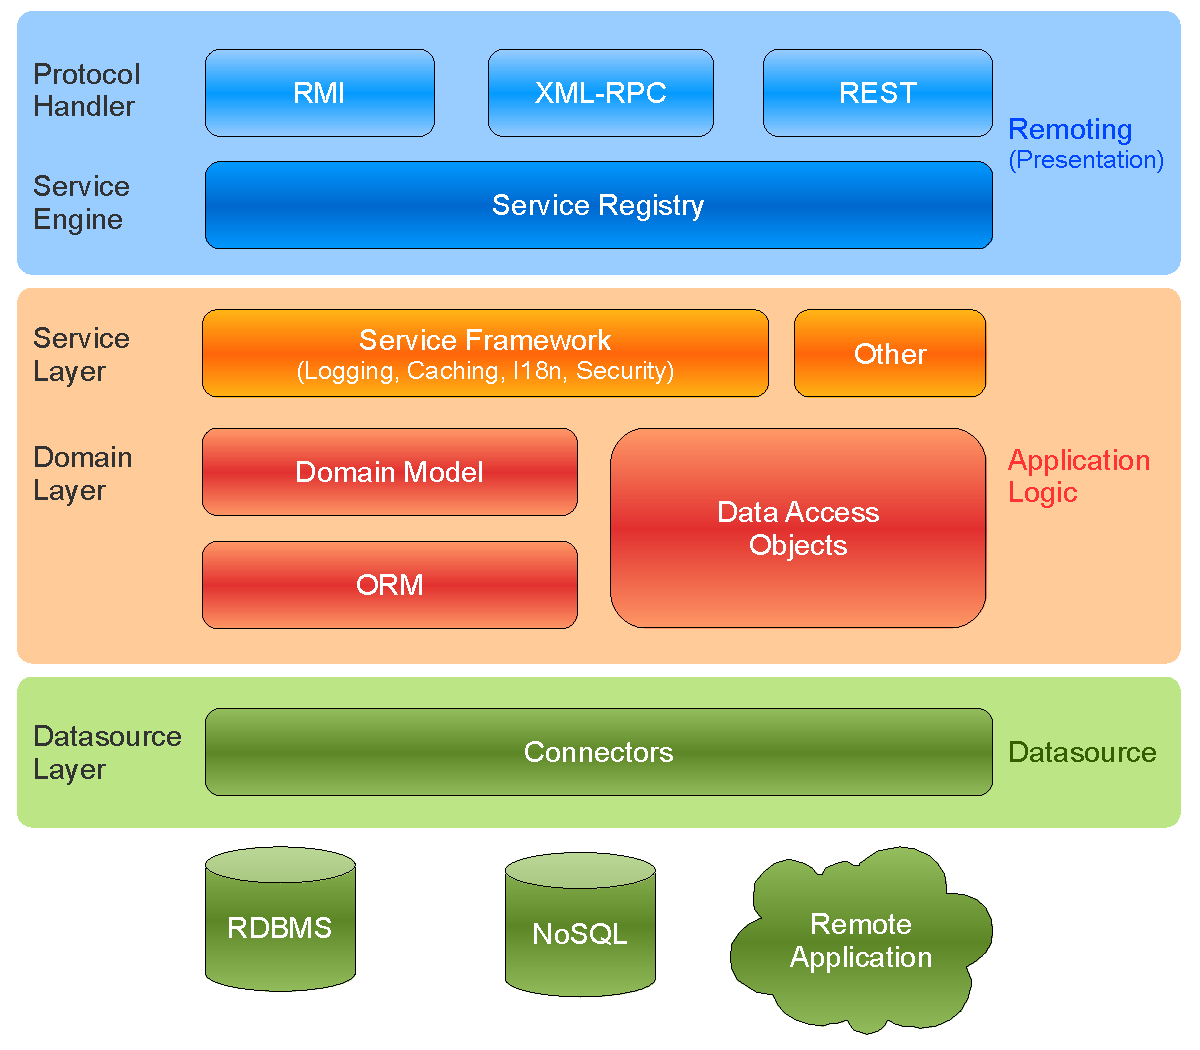
\includegraphics[width=\linewidth]{images/overviews/overview}}
	\caption{Architekturübersicht}
	\label{ill:overview}
\end{figure}